\documentclass[12pt]{article}
\usepackage[top=1in, bottom=1in, left=1in, right=1in]{geometry}

\usepackage{setspace}
\onehalfspacing

\usepackage{amssymb}
%% The amsthm package provides extended theorem environments
\usepackage{amsthm}
\usepackage{epsfig}
\usepackage{times}
\renewcommand{\ttdefault}{cmtt}
\usepackage{amsmath}
\usepackage{graphicx} % for graphics files

% Draw figures yourself
\usepackage{tikz} 

% writing elements
\usepackage{mhchem}

% The float package HAS to load before hyperref
\usepackage{float} % for psuedocode formatting
\usepackage{xspace}

% from Denovo Methods Manual
\usepackage{mathrsfs}
\usepackage[mathcal]{euscript}
\usepackage{color}
\usepackage{array}

\usepackage[pdftex]{hyperref}
\usepackage[parfill]{parskip}

% math syntax
\newcommand{\nth}{n\ensuremath{^{\text{th}}} }
\newcommand{\ve}[1]{\ensuremath{\mathbf{#1}}}
\newcommand{\Macro}{\ensuremath{\Sigma}}
\newcommand{\rvec}{\ensuremath{\vec{r}}}
\newcommand{\omvec}{\ensuremath{\hat{\Omega}}}
\newcommand{\sigs}{\ensuremath{\Sigma_s(\rvec,E'\rightarrow E,\omvec'\rightarrow\omvec)}}
\newcommand{\el}{\ensuremath{\ell}}
\newcommand{\sigso}{\ensuremath{\Sigma_{s,0}}}
\newcommand{\sigsi}{\ensuremath{\Sigma_{s,1}}}
%---------------------------------------------------------------------------
%---------------------------------------------------------------------------
\begin{document}
\begin{center}
{\bf NE 250, F15 \\
September 21, 2015}
\end{center}

Please note: I posted a fairly different derivation of the TE and DE on the class page (called 15-19-te-de). This is how I taught it in NE 155 and I think it's both clearer and more thorough. This could be useful as you sort through things. 

Last class we started with the two equations we had arrived at using the $P_1$ approximation: one for scalar flux and one for current. We then made a few simplifications / assumptions:
\begin{itemize}
\item The angular flux can be represented by \textbf{linearly anisotropic} angular dependence (that is the $P_1$ expansion). 
The approximation is valid away from boundaries, away from neutron sources and sinks, and in media that are not highly absorbing.
\item one speed.
\item isotropic source.
\item neutron current density changes slowly on a time scale compared to the mean collision time:
\begin{align*}
\frac{1}{|\vec{J}(\rvec,t)|}&\frac{\partial\vec{J}(\rvec,t)}{\partial t} \ll v\Sigma_t \\ \frac{1}{|\vec{J}(\rvec,t)|}&\frac{\partial\vec{J}(\rvec,t)}{\partial t}\approx 0
\end{align*}
The collision frequency $v\Sigma_t$ is typically on the order of $10^5$ sec$^{-1}$ or larger, so only an extremely rapid time variation of the current would invalidate this assumption (such rapid changes are very rarely encountered in reactor dynamics).
\end{itemize}

All of that got us to \textit{Fick's law} and \textit{the one-speed diffusion equation}.  
%
\begin{equation*}
\frac{1}{v}\frac{\partial\phi(\rvec,t)}{\partial t} = S(\rvec,t) - \Sigma_a(\rvec)\phi(\rvec,t) + 
\nabla\cdot[D(\rvec)\nabla\phi(\rvec,t)],
\end{equation*}
%
We talked about the boundary conditions necessary to solve this equation last time. 

--------------------------------------------------------------\\
Now, let's revisit the the energy-dependent $P_1$ equations:

\begin{align*}
\frac{1}{v}\frac{\partial\phi(\rvec,E,t)}{\partial t} &= S(\rvec,E,t) + 
\int^{\infty}_0dE'\:\Sigma_s(\rvec, E'\rightarrow E)\phi(\rvec,E',t) - 
\Sigma_t(\rvec,E)\phi(\rvec,E,t) - \nabla\cdot\vec{J}(\rvec,E,t)\\
%
\frac{1}{v}\frac{\partial \vec{J}(\rvec,E,t)}{\partial t} &= S_1(\rvec,E,t) + 
\int^{\infty}_0dE'\:\bar{\mu_0}\Sigma_s(\rvec,E'\rightarrow E)\vec{J}(\rvec,E',t) - 
\Sigma_t(\rvec,E)\vec{J}(\rvec,E,t) - \frac{1}{3}\nabla\phi(\rvec,E,t)
\end{align*}

From the $\frac{1}{|\vec{J}(\rvec,t)|}\frac{\partial\vec{J}(\rvec,t)}{\partial t}\ll v\Sigma_t$ 
assumption, $\frac{1}{v}\frac{\partial\vec{J}(\rvec,t)}{\partial t} = 0$.

From the isotropic source assumption, $S_1(\rvec,E,t) = 0$.

The assumption of isotripic scattering would give $\Sigma_{s1}(E' \rightarrow E)=0$, which results in
\[\vec{J}(\vec{r}, E, t) \approx - \frac{1}{3 \Sigma_t(\vec{r}, E)}\nabla \phi(\vec{r}, E, t)\:. \]
However, the assumption of isotropic scattering is often too strong for most reactor calculations.

Instead, we can simply define an energy-dependent diffusion coefficient as
\[D(\vec{r}, E) = \frac{1}{3} \biggl[ \Sigma_t(\vec{r}, E) - \frac{\int_0^{\infty} dE' \: \Sigma_{s1}(\vec{r},E' \rightarrow E)J_i(\vec{r}, E', t)}{J_i(\vec{r}, E', t)}\biggr]^{-1}\:,\]
which would automatically yield
\[\vec{J}(\vec{r}, E, t) = -D(\vec{r},E)\nabla \phi(\vec{r}, E, t)\:.\]
[Note that $i = x,y,z$. We need to do each vector component separately since $D$ is a scalar, and then recombine to get $\vec{J} = J_x \Omega_x + J_y \Omega_y + J_z \Omega_z$.]\\
This is artificial because $D$ actually depends on $\vec{J}$.

One common way to avoid this is to neglect the anisotropic contribution to energy transfer in the scattering collision by saying
\[\Sigma_{s1}(\vec{r},E' \rightarrow E) = \Sigma_{s1}(\vec{r},E) \delta(E' - E)\]
such that
\[\int_0^{\infty} dE' \: \Sigma_{s1}(\vec{r},E' \rightarrow E)J_i(\vec{r}, E', t) = \bar{\mu_0} \Sigma_s(\vec{r},E) J_i(\vec{r}, E, t)\:.\]
And all of that gives
\[D(\vec{r}, E) = \frac{1}{3} \bigl[\Sigma_t(\vec{r}, E) - \bar{\mu_0} \Sigma_s(\vec{r}, E) \bigr]^{-1}\:.\]

Plugging this into the first $P_1$ equation gives

\begin{equation*}
\frac{1}{v}\frac{\partial\phi(\rvec,E,t)}{\partial t} = S(\rvec,E,t) + 
\int^{\infty}_0dE'\:\Sigma_s(\rvec,E'\rightarrow E)\phi(\rvec,E',t) - 
\Sigma_t(\rvec,E)\phi(\rvec,E,t) + \nabla\cdot[D(\rvec,E)\nabla\phi(\rvec,E,t)]
\end{equation*}


--------------------------------------------------------------\\
Now, let's make the \emph{one-group} (not one-speed) assumption. This means that we will integrate the
entire equation over all energy space $[\int_0^{\infty}dE(\cdot)]$; we will often weight this integration with the flux.

``Group constants" are defined as follows (note that subscripts are now group number, not expansion coefficient or time index):

\begin{equation*}
\Sigma_{t,1}(\rvec)=\frac{\int_0^{\infty}dE\Sigma_t(\rvec,E)\phi(\rvec,E,t)}{\int_0^{\infty}dE\phi(\rvec,E,t)}
= \text{effective cross section}
\end{equation*}

\begin{equation*}
\phi_1(\rvec,t) = \int_0^{\infty}dE\phi(\rvec,E,t) = \text{group flux}
\end{equation*}

Thus, $\int_0^{\infty}dE\Sigma_t(\rvec,E)\phi(\rvec,E,t) = \Sigma_{t,1}(\rvec)\phi_1(\rvec,t)$.

\begin{equation*}
\int_0^{\infty}dE\frac{1}{v}\frac{\partial\phi(\rvec,E,t)}{\partial t} = 
\frac{1}{v_1}\frac{\partial \phi_1(\rvec,t)}{\partial t}, 
\text{ where } \frac{1}{v_1} = \frac{\int_0^{\infty}dE\frac{1}{v}\phi(\rvec,E,t)}{\phi_1(\rvec,t)}
\end{equation*}

\begin{equation*}
\int_0^{\infty}dES(\rvec,E,t) = S_1(\rvec,t)
\end{equation*}

\begin{equation*}
\int_0^{\infty}dE\int_0^{\infty}dE'\Sigma_s(\rvec,E'\rightarrow E)\phi(\rvec,E',t) =
\int_0^{\infty}dE'\Sigma_s(\rvec,E')\phi(\rvec,E',t) = \sigsi\phi_1
\end{equation*}

\begin{equation*}
\int_0^{\infty}dE\nabla\cdot[D(\rvec,E)\nabla\phi(\rvec,E,t)]=\nabla\cdot[D_1(\rvec)\nabla\phi_1(\rvec,t)]
\end{equation*}

Note that although the subscripts used here for the one-group approximation are the same as those used in
the $P_1$ approximation derivation, the quantities are not the same. Combining all of the above terms, we
have

\begin{equation*}
\frac{1}{v_1}\frac{\partial \phi_1(\rvec,t)}{\partial t} = S_1(\rvec,t) - 
\Sigma_{a,1}(\rvec)\phi_1(\rvec,t) + \nabla\cdot[D_1(\rvec)\nabla\phi_1(\rvec,t)]
\end{equation*}

This is the \emph{one-group} diffusion equation.

--------------------------------------------------------------\\
We were talking about currents and boundary conditions at the end of class, so let's quickly revisit that. 

For the TE, the one-group vacuum boundary condition is $\varphi_1 (\vec{r}_s, \omvec, t) = 0 \quad \text{for }\omvec \cdot d\vec{S} < 0\:, \forall \rvec_s \text{ on } \vec{S}$.

We will seek to satisfy this in an integral sense for the diffusion equation, remembering that
\begin{equation*}
J_{\pm,1} = \int_{2\pi^{\pm}}d\omvec\:\omvec\cdot\hat{e}_s\varphi_1(\rvec,E,\omvec,t)\:.
\end{equation*}
Therefore, $J_{-,1}(\rvec_s,t) = 0$.

Using the $P_1$ approximation for this, then
\[J_{-,1} = \int_{2\pi^{-}}d\omvec\:\omvec\cdot\hat{e}_s\varphi_1(\rvec,E,\omvec,t) \approx \frac{1}{4}\phi_1(\rvec, t) + \frac{D_1(\rvec)}{2}\hat{e}_s \cdot \nabla \phi_1(\rvec, t) = 0\:.\]


In 1D,
\begin{equation*}
J_{-,1}(z_s,t) = \frac{1}{4}\phi_1(z_s,t) + \frac{D_1(z_s)}{2}\frac{d\phi_1(z_s,t)}{dz}\Bigr|_{z_s} = 0
\end{equation*}

\begin{equation*}
\frac{d\phi_1(z_s,t)}{dz}\Bigr|_{z_s} = \frac{-\phi_1(z_s,t)}{2D_1(z_s)}
\end{equation*}

In order to use the diffusion approximation, we must accept that the above solution at the vacuum is wrong, necessitating the introduction of an extrapolation distance:

\begin{equation*}
\tilde{z}_s = z_s + 2D_1(z_s)
\end{equation*}

We therefore typically use the boundary condition $\phi(\tilde{z}_s) = 0$. 
Note that that a more accurate extrapolation distance that is obtained from transport theory is $\tilde{z}_s = z_s + z_0; z_0 = 0.7104 \lambda_{tr}$.

\begin{figure}
    \begin{center}
    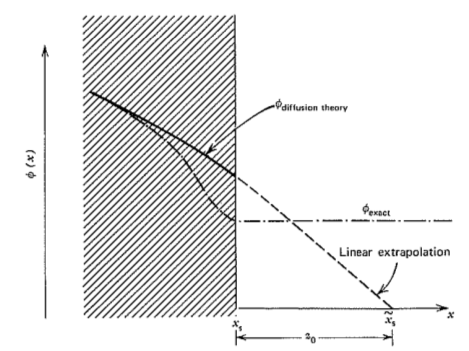
\includegraphics[keepaspectratio, width = 3 in]{extrapolation}
    \end{center}
    \label{fig:phase_space}
\end{figure}

There are a few other types of conditions we might encounter or apply:
\begin{itemize}
\item We know that the flux must be nonnegative, finite, and real. 
\item Symmetry often lets us eliminate solutions that don't make physical sense (e.g.\ at the centerline of a slab we know that $\phi(-x) \neq - \phi(x)$). 
\item We use \textit{unit cells} or \textit{control cells} that are repeated in a regular fashion. 
One can argue that there should be no net transfer of neutrons between cells, so $\vec{J}(\rvec)$ vanishes on those boundaries.
\item When these cells are near strong absorbers, we usually end up doing a transport correction to get more accurate boundary conditions. 
(Note that within the derivation of the DE, we used transport corrections in some occasions to make it more accurate. )
\end{itemize}

\begin{figure}
    \begin{center}
    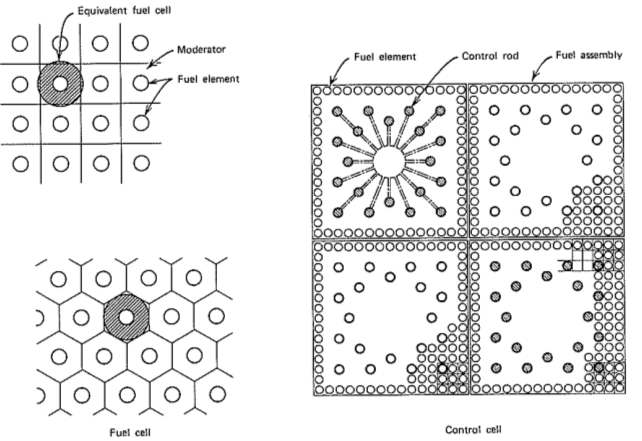
\includegraphics[keepaspectratio, width = 5 in]{unit-cell}
    \end{center}
    \label{fig:phase_space}
\end{figure}

-------------------------------------\\
A quick one-speed diffusion summary:
\[\frac{1}{v} \frac{\partial \phi}{\partial t} = S(\rvec, t) + \Sigma_a(\rvec) ]\phi(\rvec, t) + \nabla \cdot D(\rvec) \nabla \phi(\rvec, t)\:.\]

Where
\begin{itemize}
\item $\phi(\rvec, 0) = \phi_0(\rvec) \: \forall \: \rvec$
\item $\phi(\tilde{\rvec_s}, t) = 0$ or $J_-(\rvec_s, t) = 0$; (free surface)
\item $\phi$ and the normal component of $\vec{J}$ are continuous across surfaces
\item $0 \leq \phi(\rvec, t) < \infty$ (except near localized sources).
\item $D = \lambda_{tr}/3 = [3(\Sigma_{tr} - \bar{\mu_0}\Sigma_s)]^{-1}$
\item $\rvec_0 = 0.7104 \lambda_{tr}$.
\end{itemize}
This equation is \textbf{parabolic}. Equations of this form apply to heat conduction, gas diffusion, the wave function, etc.

If we are in a situation where the materials are homogeneous, we drop $\rvec$ dependence in all of the coefficients (we can then bring the $\nabla$ inside the $D$). 
We also frequently neglect time dependence. 
In this case:
%
\begin{align*}
-D \nabla^2 \phi(\rvec) &+ \Sigma_a \phi(\rvec) = S(\rvec) \\
\nabla^2 \phi(\rvec) &- \frac{1}{L^2}\phi(\rvec) = \frac{S(\rvec)}{D}
\end{align*}
this second equation is in \textit{Helmholtz form}; which we use to take advantage of common mathematical solution techniques.
Note that $L$ is the neutron diffusion length
\[L \equiv \sqrt{\frac{D}{\Sigma_a}}\:,\]
which is a measure of how far neutrons diffuse before they are absorbed.

\end{document}
